\documentclass[11pt,letterpaper,notitlepage]{report}
\usepackage[latin1]{inputenc}
\usepackage{amsmath}
\usepackage{amsfonts}
\usepackage{amssymb}
\usepackage{fancyhdr}
\newcommand{\field}[1]{\mathbb{#1}}
\renewcommand{\labelenumi}{\alph{enumi})}
\usepackage{tikz}
\usepackage{fancybox}
\title{Minesweeper Solver Analysis}
\author{Brian Stack, bis12@case.edu}
\date{\today}
\usepackage[small,bf]{caption}
\usepackage{subfigure}
\usepackage{wrapfig}
\usepackage{fullpage}
\usepackage{tikz}
\usepackage{tikz-qtree}



\begin{document}
\maketitle
\section*{Analysis of Game}
\begin{enumerate}
\item 
\begin{align*}
C = \{ (V_1, V_2) &= V_1 + V_2 = 1,\\
       (V_3, V_4) &= V_3 + V_4 = 1,\\
       (V_1, V_2, V_3, V_4, V_5) &= V_1 + V_2 + V_3 + V_4 + V_5 = 2\}
\end{align*}
\item In the tree, if any nodes did not branch for their children, I collapsed them into one to save space.\\ %CHECK THIS AND POSSIBLY IMPROVE THIS LATER
\begin{center}
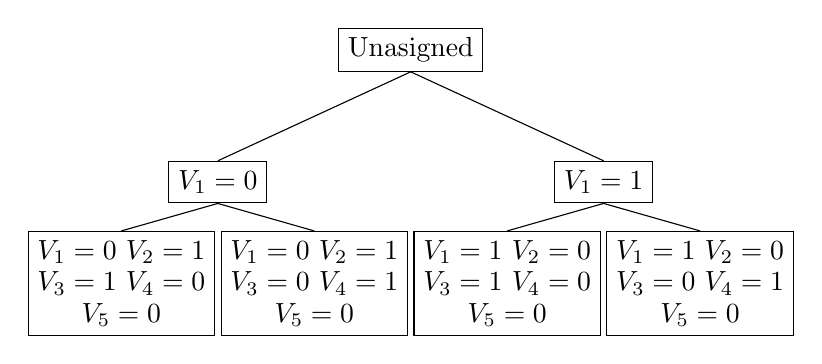
\begin{tikzpicture}
\tikzset{level distance=48pt}
\tikzstyle{every node}=[rectangle,draw]
\Tree [.Unasigned [.{$V_1 = 0$}
[.\shortstack{$V_1 = 0$ $V_2 = 1$\\ $V_3 = 1$ $V_4 = 0$\\ $V_5 = 0$} ]  
[.\shortstack{$V_1 = 0$ $V_2 = 1$\\ $V_3 = 0$ $V_4 = 1$\\ $V_5 = 0$} ] 
] [.{$V_1 = 1$} 
[.\shortstack{$V_1 = 1$ $V_2 = 0$\\ $V_3 = 1$ $V_4 = 0$\\ $V_5 = 0$} ]  
[.\shortstack{$V_1 = 1$ $V_2 = 0$\\ $V_3 = 0$ $V_4 = 1$\\ $V_5 = 0$} ] 
] ]   
\end{tikzpicture}
\end{center}
It does provide an optimal next choice.
\item All four possibilities are enumerated below\\
\begin{tabular}{ccccc}
$V_1$&$V_2$&$V_3$&$V_4$&$V_5$\\\hline
0&1&1&0&0\\
0&1&0&1&0\\
1&0&1&0&0\\
1&0&0&1&0
\end{tabular}
\item $V_5$ cannot possibly reveal a mine because in no possible configuration does it contain one.
\item DOOOOOOOO THHHHHHHHHHHHHHIIIIIIIIIIIIS LATEDR
\end{enumerate}
\section*{Observations on Solutions}
\begin{enumerate}
\setcounter{enumi}{2}
\item ababab
\end{enumerate}
\end{document}





